\section{\tc Design}

We now present our \tc architecture. First, we present a strawman architecture that illustrates some of the technical challenges that arise in the design of \tc. We then present our \tc architecture, first describing the interface available to a relying contract \reqcont, then the back end, and finally an overview of the security model.

\subsection{Strawman architecture}

A naive strawman solution is the following:
\begin{itemize}[leftmargin=5mm]
\item
{\bf Monitor and relay.}
The Town Crier relay $\relay$    
monitors the blockchain for 
contracts that require authenticated data feeds (e.g., those
that make calls to $\tcont$).

Suppose a contract requires 
an authenticated 
data feed with the following parameters ${\sf params} := (\weburl, \pkurl, T)$,
where $\weburl$ denotes the site's URL,
$\pkurl$ denotes the site's cryptographic 
identity, and $T$ denotes a time at which the site should be scraped.
Town Crier's relay $\relay$ will then send
a request ${\sf params}$ 
to the SGX enclave at time $T$.
\item
{\bf Securely fetch feed.}
The SGX enclave will now fetch the webpage at $\weburl$ by establishing
an HTTPS secure channel with 
the cryptographic entity $\pkurl$.
After fetching the contents of the page, 
the enclave parses the webpage's contents and extracts the datagram requested
denoted ${\sf data}$.
Finally, the SGX enclave produces an attestation 
vouching for the tuple $(\weburl, \pkurl, T, {\sf data})$.
Specifically, note that the SGX enclave also vouches
for the time $T$ at which the data source is fetched.
\item
{\bf Verify}.
Now, the blockchain contract $\tcont$ verifies the attestation
produced by the SGX enclave, and 
if verification succeeds, proceeds to make use of 
the resulting datagram ${\sf data}$.
\end{itemize}

\paragraph{Problems with the strawman scheme.}
The above strawman scheme has a few drawbacks. 

First, the blockchain contract
$\tcont$ must verify an SGX group signature.  
This could be wasteful in terms of on-chain cost, 
\elaine{things like on-chain cost and gas should be mentioned in a 
background section}
since the group signature verification requires inputing 
to $\tcont$ the latest revocation list 
for SGX's group signature scheme.
Moreover, 
this also gives rise to a practical engineering issue if we
were 
to build $\tcont$ atop Ethereum,
since implementing group signature verification in Ethereum's Serpent
or Solidity language is non-trivial and wasteful in terms of gas.

Second, for the SGX enclave to  
attest to the time $T$ at which the data source is fetched, 
we need the SGX enclave to provide a trusted clock that provides absolute time. 
Although Intel's SGX provides a 
trusted clock API, the trusted clock does not provide absolute time,
but rather, relative time with respect to a certain reference point.  
Therefore, it is not immediately clear how to realize 
a trusted absolute clock.


\iffalse

At first glance, a simple architecture might be envisioned in which \tc has no explicit blockchain presence such as a smart contract or account. Instead, the \tc host scrapes the blockchain, searching for any contract \reqcont whose state contains a datagram request or an attestation request. The \tc sends datagrams or fresh attestations to \reqcont accordingly. A trusted component, which we will call an \encname, runs in an SGX enclave. To ensure data integrity, the \encname obtains data from data sources via an HTTPS. This general design approach would have a number of benefits, including: no need for contracts to send explicit requests to \tc (saving gas and potentially complexity), ensuring that a relying contract \reqcont consumes only fresh SGX attestations from \tc, and conceptual simplicity.

This approach, however, is unworkable for several reasons. First, it is desirable for \tc to accept on-blockchain payments via a smart contract in order to permit payment in the system's cryptocurrency (e.g., Ether) and to ensure a {\em fair exchange} between payments and datagrams. Even a not-for-profit \tc service might accept small gas payments to cover the cost of datagram transmission. Without enforcement of fair exchange, relying contracts or the \tc service would risk being defrauded by the other party. Second, because an SGX enclave does not have direct network connectivity (and our adversarial model includes general network adversaries), an adversarial OS on the SGX host could {\em corrupt blockchain data furnished to the \encname}, resulting in the construction of incorrect datagrams. (Datagram specifications could be sent from the \encname to \reqcont for verification, but the resulting, weak security model for \tc would create unneeded complexity for relying contract creators.) It is to address these two concerns that we design \tc with a blockchain front end in the form of a contract \tcont.

A third reason for the infeasibility of our strawman architecture results from the limitations in the current specification of Ethereum.In Ethereum, opcodes for in-contract cryptographic operations are very limited and do not currently support any form of public-key cryptography, let alone the proprietary EPID group-signature scheme present in SGX attestations. (Digital signatures are supported only for messages from non-contract accounts.) On-blockchain verification of attestations is feasible in principle, as the Ethereum virtual machine is Turing-complete, but would be prohibitively expensive for contracts, imposing exorbitant gas costs. For this reason, our \tc design favors off-chain verification of attestations.
\fi

\subsection{The \tc interface}

The blockchain interface to \tc is the smart contract \tcont. \tcont is designed to present a simple API to a relying contract / requester \reqcont. \reqcont sends to \tcont a specification of the datagram it is requesting, along with payment. The datagram specification includes the data being sought and may also include datagram parameters, such as the time at which the data should be retrieved, the target source or sources, and so forth. \tcont simply returns the requested data to \reqcont. The interaction between \reqcont and \tcont takes place entirely on the blockchain.

The complexity of \tc resides primarily in its backend, which must monitor, keep track of, and fulfill datagram requests passing from requesters through \tcont. Additionally, \tc supports an off-chain service, specifically, a web service, to furnish SGX attestations to clients.

\subsection{The \tc architecture}

The \tcs system includes three main components: The \tcontract, the \encname, and the \medname. The \encname and \medname reside on the \tc server, while the \tcontract resides on the blockchain. An architectural schematic showing the roles of these components is given in Figure~\ref{fig:overview}.

\vspace{-2mm}
\begin{figure}[h!]
\centering
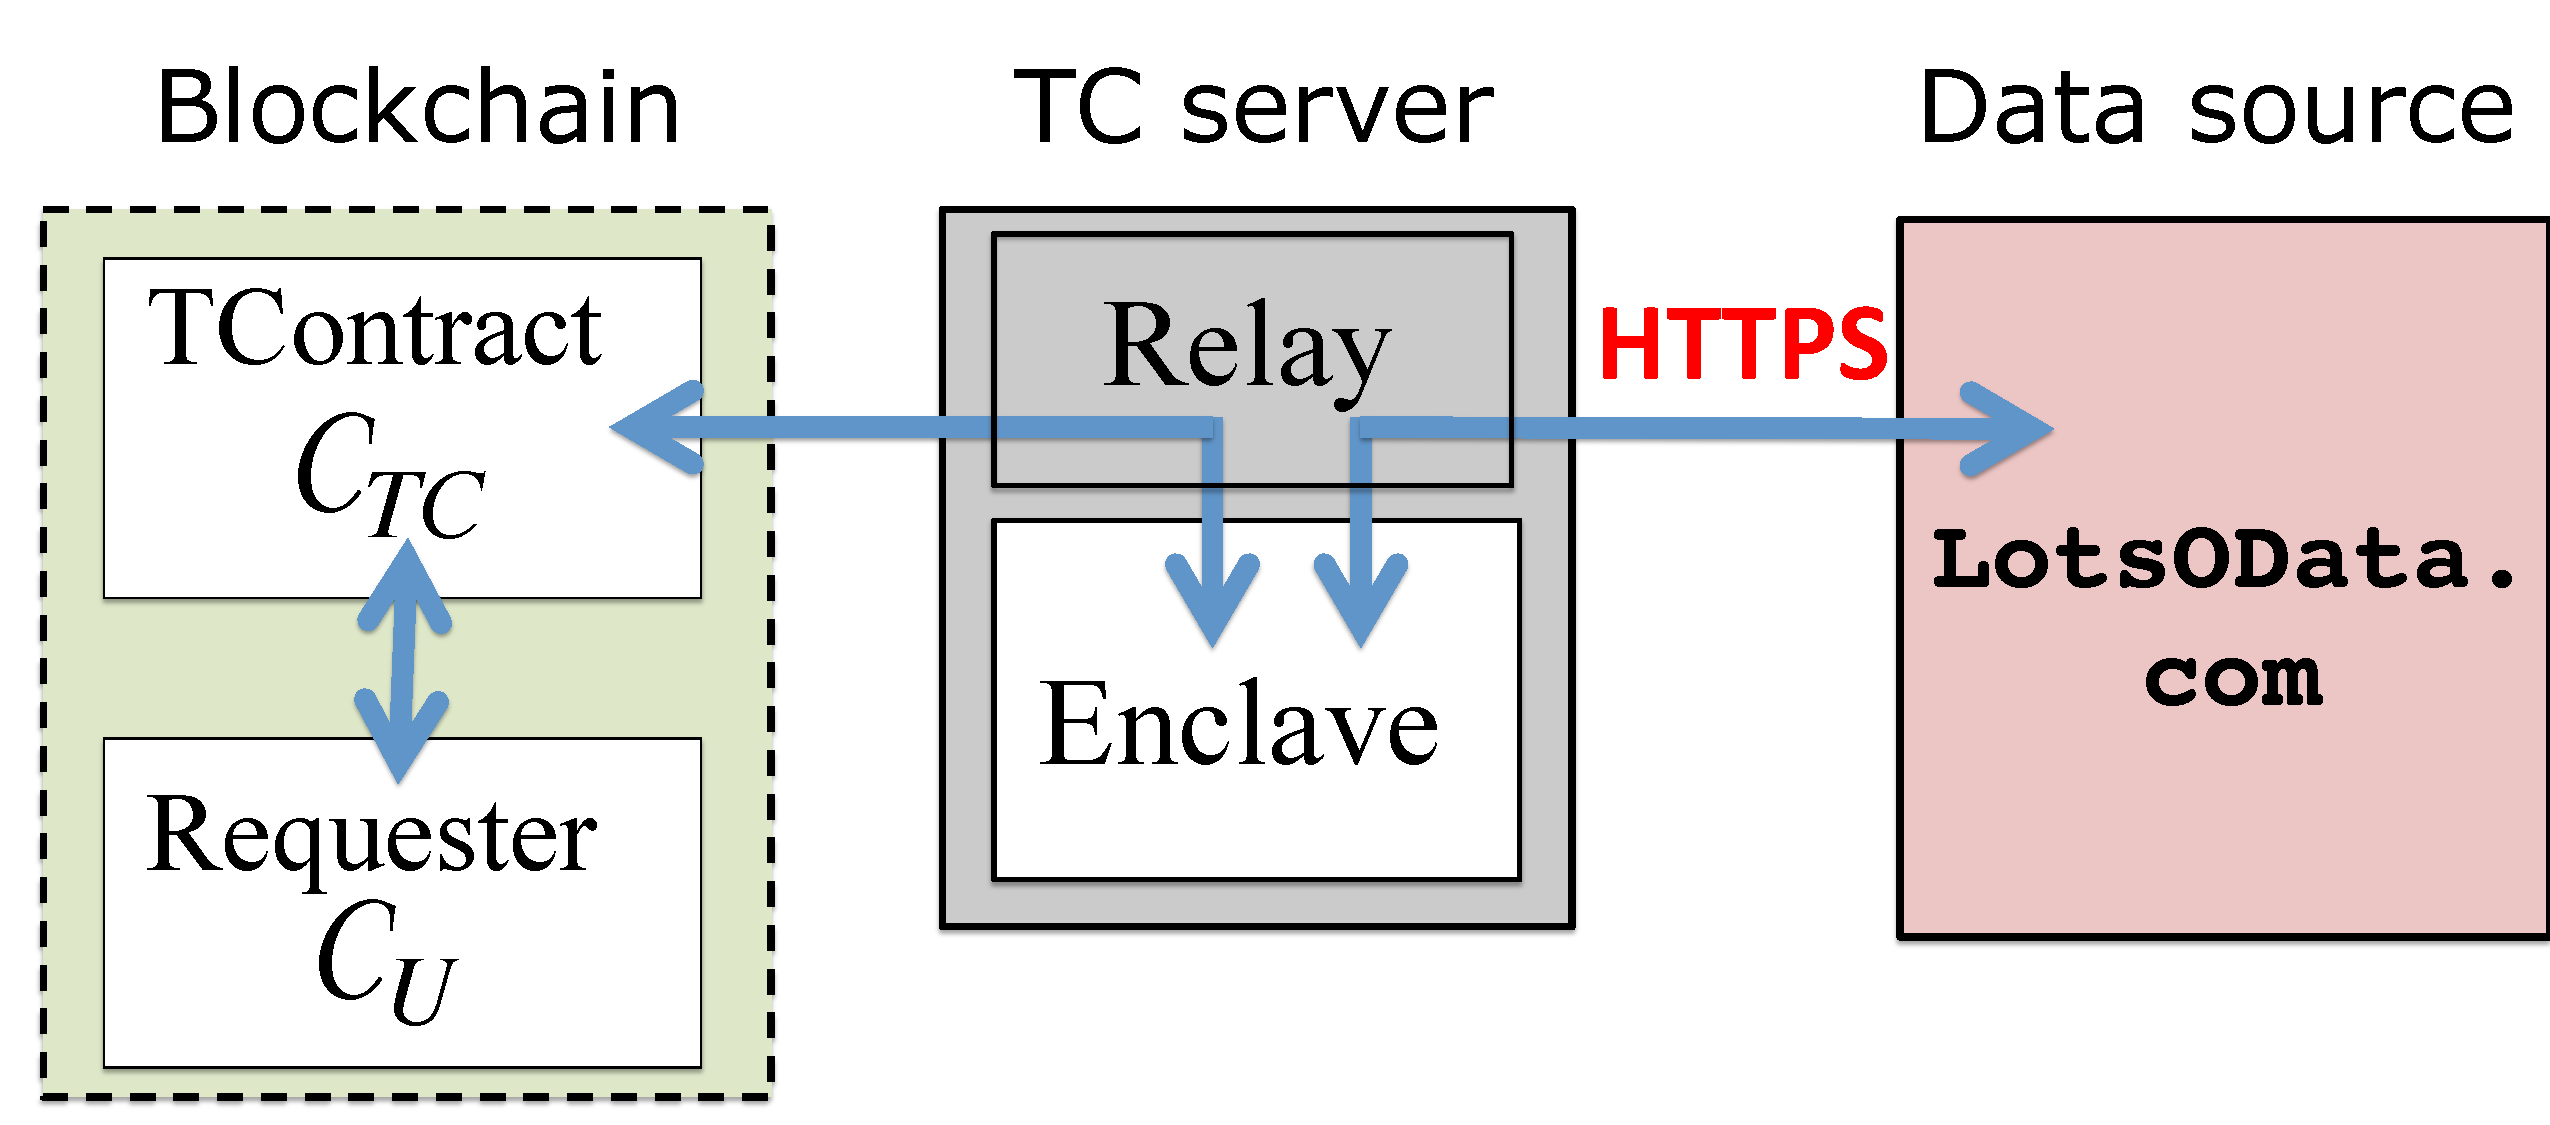
\includegraphics[width=\columnwidth]{figures/OverviewFig}
\caption{{\bf Basic Town Crier architecture.}}
\label{fig:overview}
\end{figure}
\vspace{-2mm}

\paragraph{The \tcontract (\tcont).} The \tcontract (denoted by \tcont) is a smart contract that acts as the blockchain front-end of the \tc service, and thus an interface between relying contracts and \tc. It accepts datagram requests from a requester \reqcont and returns corresponding datagrams from \tc. Additionally, the \tcontract manages \tc monetary resources, which in Ethereum take the form of ether (money) and gas (``fuel'' for contracts). 

\paragraph{The \encname.}
The \encname ingests and fulfills datagram requests from the blockchain. To obtain the data for inclusion in datagrams, it queries external data sources, specifically HTTPS-enabled internet services. It returns a datagram to a requesting contract \reqcont as a digitally signed blockchain message. The \encname runs in an SGX enclave, and is thus secured against an adversarial OS as well as other process on the host. 

\paragraph{The \medname.} As an enclave process, the \encname lacks direct network access. Thus the \medname handles bidirectional network traffic on behalf of the \encname. Specifically, the \medname provides network connectivity from the \encname to three different types of entities: 

\begin{enumerate}
\item {\em The Blockchain (the Ethereum system):}  The \medname scrapes the blockchain in order to monitor the state of the \tcontract  \tcont. In this way, it performs implicit message passing from \tcont to the \encname, as neither component itself has network connectivity. Additionally, the \medname places messages emitted from the \encname (datagrams) on the blockchain.
\item {\em Clients:} The \medname runs a web server to handle off-chain service requests from clients, specifically, requests for attestations from the \encname. As we soon explain, an attestation provides a unique public key for the \encname instance to the  client and proves that the \encname is executing correct code in an enclave and that its clock is correct in terms of absolute (wall-clock time). A client that successfully verifies an attestation can then safely create a relying contract \reqcont that uses the \tc.
\item {\em Data sources:} The \medname relays traffic to and from data sources (HTTPS-enabled servers) queried by \encname. 
\end{enumerate}

The \medname is an ordinary user-space application. It does not benefit from integrity protection by trusted hardware and thus, unlike the \encname, can be subverted by an adversarial OS on the \tc server, causing network delays or failures. As we explain in detail later in the paper, however, a key design aim of \tc is that \medname should be unable to cause incorrect datagrams to be produced or users to lose money. In general, the \medname~{\em can only mount denial-of-service attacks against \tc}. 

\paragraph{End-to-end datagram processing.}

\ari{Couch in terms like strawman protocol?}
In summary, then, a datagram request is initiated by a requester \reqcont. \reqcont sends a datagram request to \tcont on the blockchain. Using network services provided by the \medname, the \encname obtains the request from the blockchain. It contacts a data source to obtain the requested data and composes a datagram, which it sends back to \reqcont.

As a simple example, \reqcont might request a stock ticker  (e.g., the price of IBM at 3 p.m. on 15 Jan 2017). The \encname would fetch the requested data from an online service (e.g., https://www.google.com/finance) and place it in a datagram for transmission via \tcont to \reqcont.

%In addition to servicing datagram requests, the \encname may be queried by a client to provide an off-chain, hardware-backed attestation $\att$ on the state of the \encname---both its executing code and its clock. It is to support this service that \medname includes a web server. We do not depict this service in Figure~\ref{fig:overview}, and defer its discussion to later in the paper.

We now make this data flow more precise. 

\subsection{Datagram processing: Data flow}

We denote a datagram instance, namely the set of message values associated with a datagram request, by $\dgi$, where $i$ is a unique instance index. (We explain in Section~\ref{sec:implementation} how this index is computed.) 

A datagram request by \reqcont takes the form of a message $\dgi.\dgreq$ to \tcont on the blockchain. This message $\dgi.\dgreq = (\dgi.\dgform, \dgi.\dgpay)$ includes both a specification $\dgi.\dgform$ of the requested datagram (e.g., a stock ticker and desired time) and a payment $\dgi.\dgpay$, which in Ethereum may include gas to cover the execution cost of the request as well as a service fee. \tcont receives a return message $\dgi.\dgret = (\dgi.\dgform, \dgi.\dgm)$ from the $\tc$ service where $\dgm$ contains the data (e.g., the desired stock ticker price). \tcont checks the consistency of $\dgi.\dgform$ on the incoming and outgoing messages, and if they match forwards $\dgi.\dgm$ to \reqcont. Where clear from context, we omit the prefix $\dgi$ from our notation.

Figure~\ref{fig:dataflow} shows the data flows involved in processing a datagram request. For simplicity, the figure omits the \medname, which is only responsible for data passing.


\begin{figure}[h!]
\centering
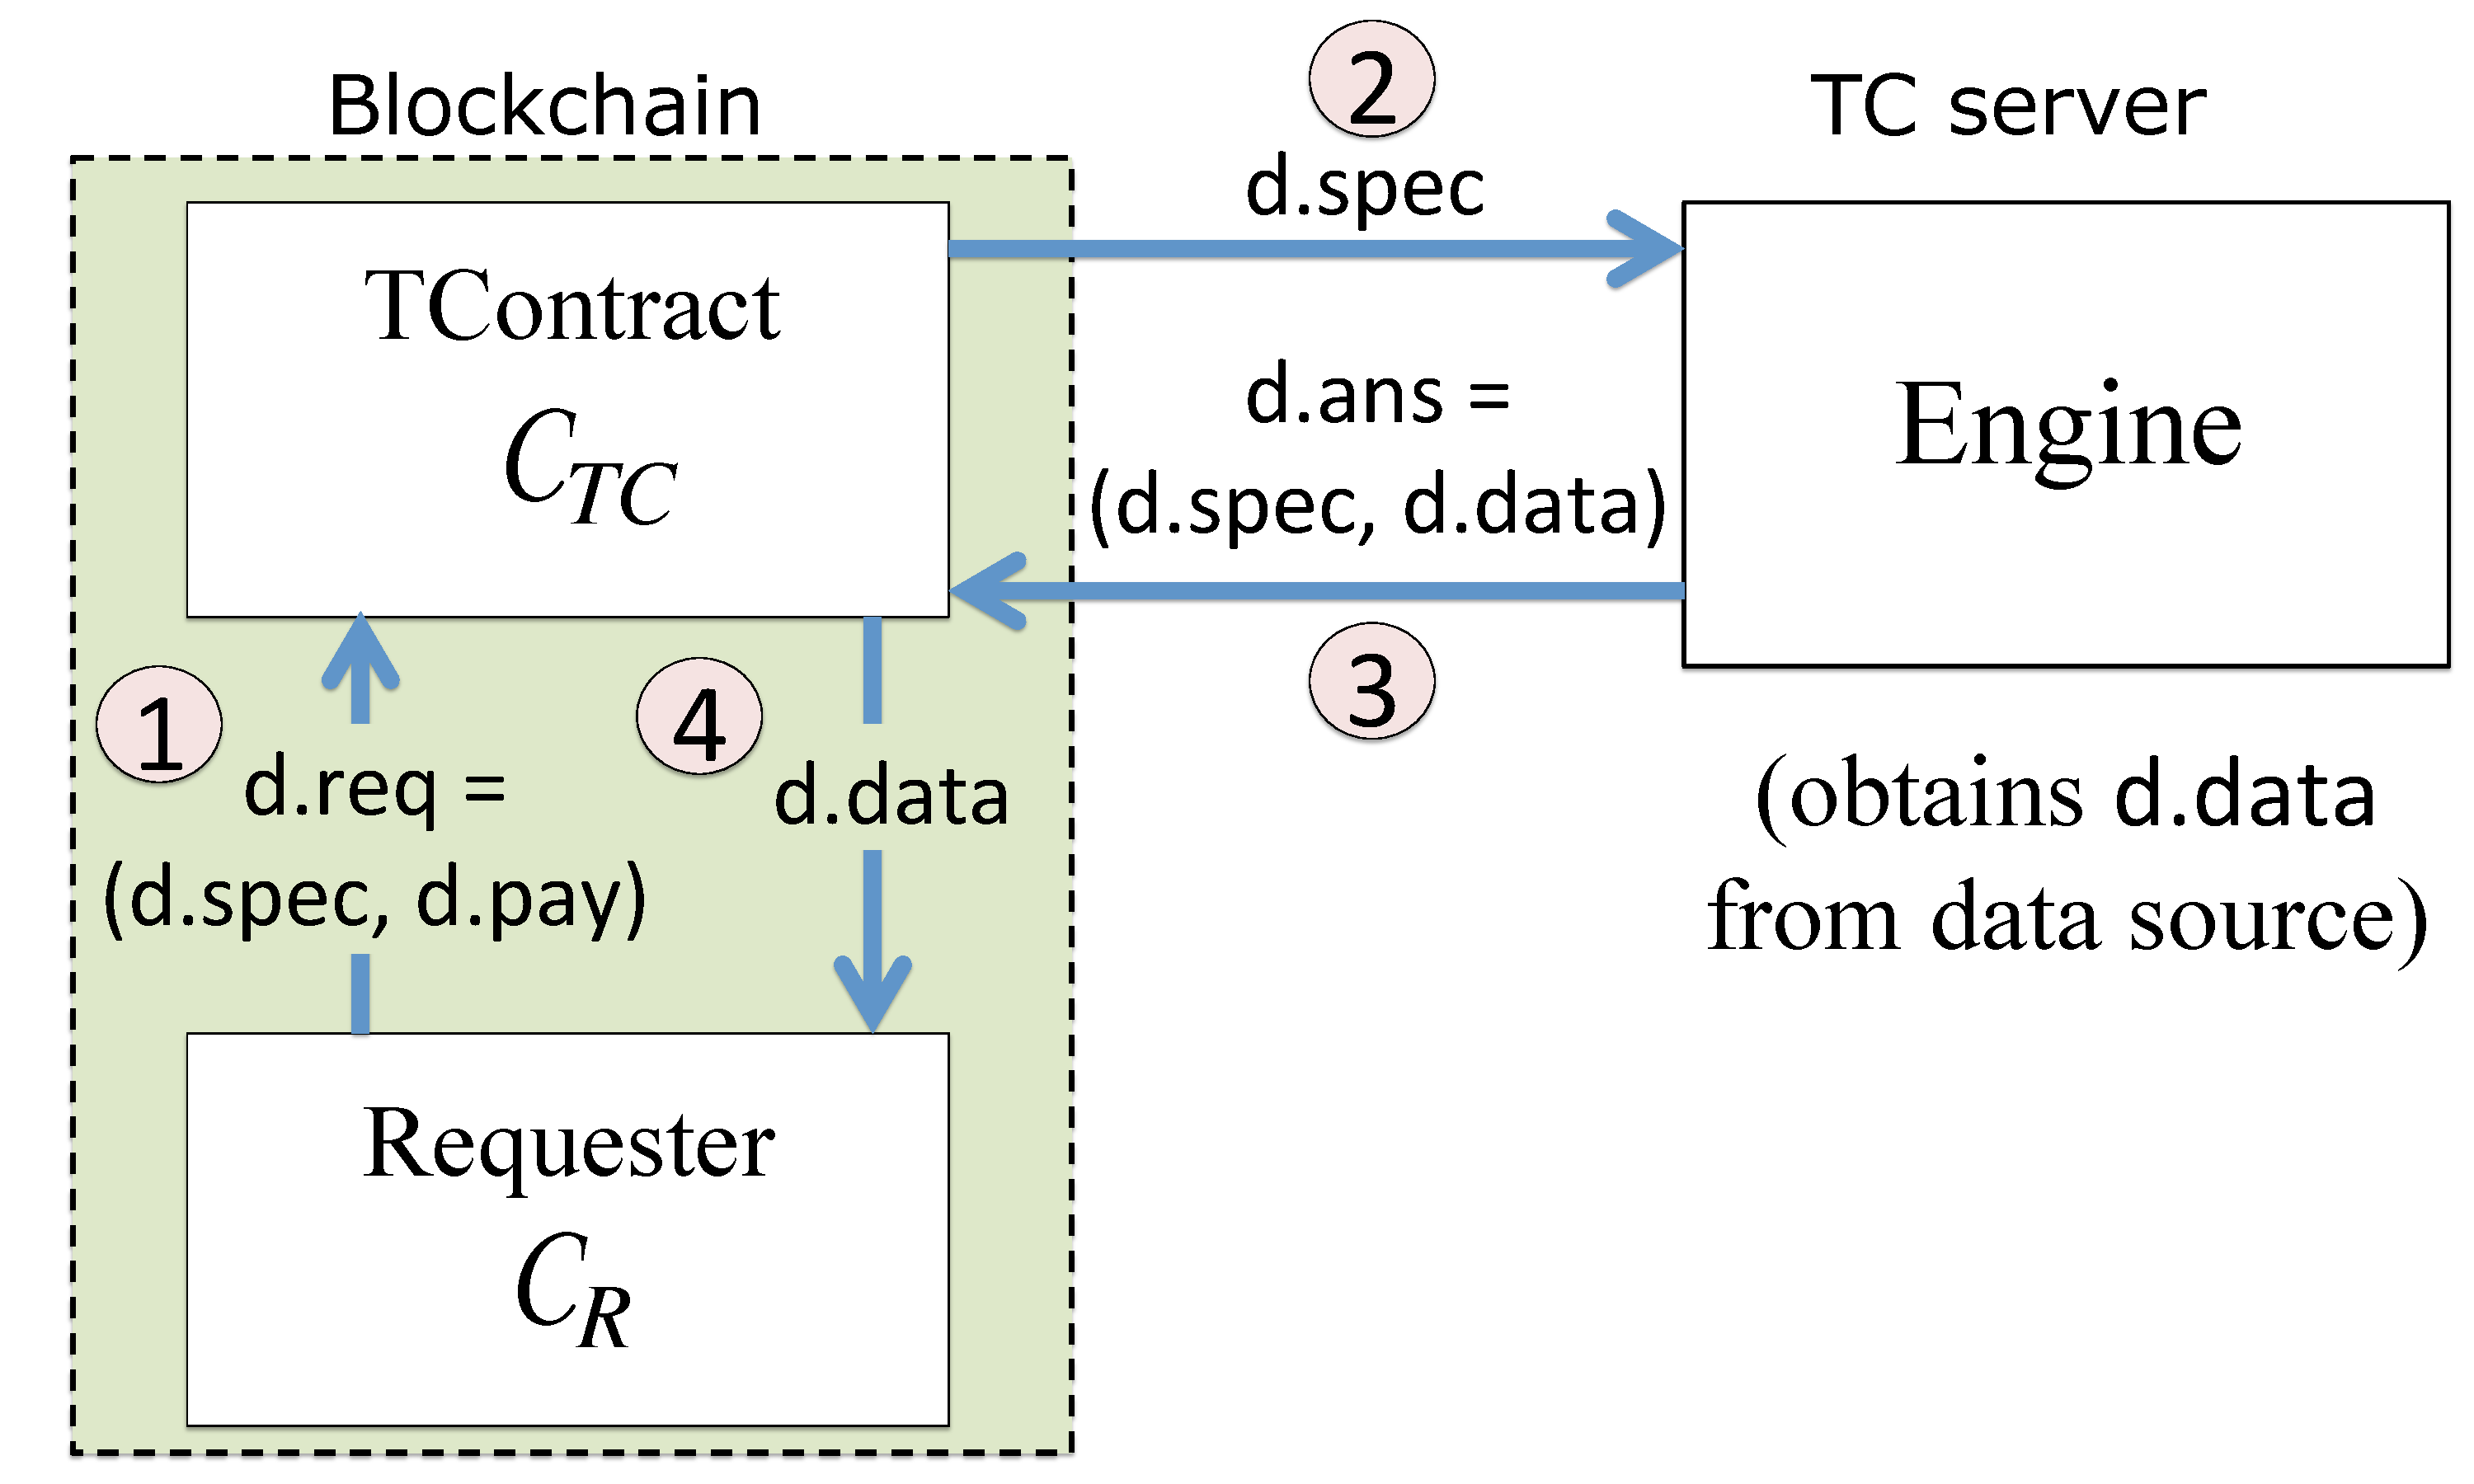
\includegraphics[width=\columnwidth]{figures/DataflowFig}
\caption{{\bf Data flows in datagram processing.}}
\label{fig:dataflow}
\end{figure}


Digital signatures are needed to authenticated messages, such as $\dgret$, entering the blockchain from an external source. We let $(\skTC, \pkTC)$ denote the private / public keypair associated with the \encname for such message authentication. For simplicity, we assume for the time that the \encname can send signed messages directly to \tcont. Later we explain how Ethereum requires a slightly different approach.

\subsection{Security model}

Here we given an overview of our security model for \tc, providing more details in our security analysis in section~\ref{}. We assume the following:

\begin{itemize}
\item {\em \encname security:} We make three assumptions about \encname : (1) \encname behaves honestly, i.e., correctly executes the \tc protocol; (2) The private key $\skTC$ is known only the \encname; and (3) The \encname has an accurate (internal) real-time clock. (Specifically, the clock is accurate to within XXX, as we show experimentally.)

These three properties are achieved under the security model presumed by SGX. Specifically, they are asserted by an SGX attestation $\att$ generated on an instance of the \encname. We make the additional simplifying assumption that an attestation remains valid throughout its lifetime of use. (Later in the paper, we discuss ways in which later incarnations of Ethereum may support fresher attestations and also issues such as SGX host revocation.)

\item {\em Network communication:} The \medname (and other untrusted components of the \tc server) can tamper with or delay communications to and from the \encname, but cannot otherwise observe or alter the behavior of the \encname. This assumption is again consistent with the SGX security model. Thus the \medname is subsumed by an adversary that controls the network. 

\item {\em Blockchain communication:} Message sources are authenticable, i.e., the originating blockchain address of a message can be correctly identified, and messages are integrity protected, but not confidential. This assumption includes messages sent from the \encname, whose public key $\pkTC$ is bound in \tc to a blockchain account. 
\end{itemize}












